\documentclass{article}
\usepackage{tikz}

\begin{document}

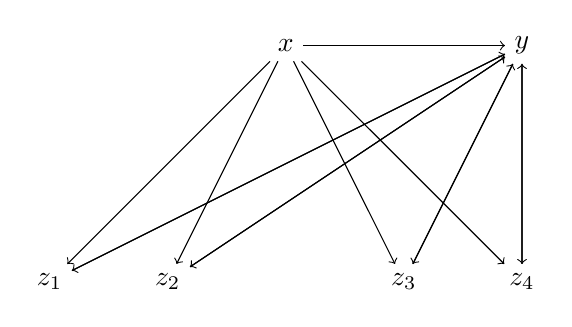
\begin{tikzpicture}[scale=1.5]
    % Define nodes
    \node (x) at (0, 0) {$x$};
    \node (y) at (2, 0) {$y$};
    \node (z1) at (-2, -2) {$z_1$};
    \node (z2) at (-1, -2) {$z_2$};
    \node (z3) at (1, -2) {$z_3$};
    \node (z4) at (2, -2) {$z_4$};

    % Draw edges
    \draw[->] (x) -- (z1);
    \draw[->] (x) -- (z2);
    \draw[->] (x) -- (z3);
    \draw[->] (x) -- (z4);
    \draw[->] (y) -- (z1);
    \draw[->] (y) -- (z2);
    \draw[->] (y) -- (z3);
    \draw[->] (y) -- (z4);
    \draw[->] (x) -- (y);
    \draw[->] (z1) -- (y);
    \draw[->] (z2) -- (y);
    \draw[->] (z3) -- (y);
    \draw[->] (z4) -- (y);
\end{tikzpicture}

\end{document}